% Usar el tipo de documento: Artículo científico.
\documentclass{beamer}

% Cargar mensajes en español.
\usepackage[spanish]{babel}

% Usar codificación utf-8 para acentos y otros.
\usepackage[utf8]{inputenc}

%Dimensiones de los márgenes.
%\usepackage[margin=1.5cm]{geometry}

% Insertar porciones de código
\usepackage{listings}

% Comenzar párrafos con separación no indentación.
\usepackage{parskip}

% Enlaces
\usepackage{hyperref}

% Usar gráficos
%\usepackage{graphicx}
%\usepackage{caption}
%\usepackage{subcaption}
\usepackage{amsmath}
\usepackage{svg}

% Fórmulas matemáticas con fuente adecuada
\usefonttheme[onlymath]{serif}

%
% Usar contenedores flotantes para figuras.
\usepackage{float}

% Carpeta de las imágenes.
\graphicspath{{img/}}
\setsvg{svgpath = img/}

% Configuración para porciones de código.
\lstset{
%	language=bash,
	basicstyle=\ttfamily\small,
%	numberstyle=\footnotesize,
%	numbers=left,
%	backgroundcolor=\color{gray!10},
%	frame=single,
	tabsize=4,
%	rulecolor=\color{black!30},
%	title=\lstname,
%	escapeinside={\%*}{*)},
	breaklines=true,
	breakatwhitespace=true,
%	framextopmargin=2pt,
%	framexbottommargin=2pt,
	extendedchars=false,
	inputencoding=utf8
}
%%%%%%%%%%%%%%%%%%%%%%%%%%%%%%%%%%%%%%%%%%%%%%%%%%%%%%%%%%%%%%%%%%%%%%%%%%%%%%%

% Propiedades
\title{Algoritmos evolutivos inspirados en computación cuántica.}

\author{Carlos Pérez Ramil (c.pramil@udc.es)\\
	Rodrigo Arias Mallo (rodrigo.arias@udc.es)}

\begin{document}

%\maketitle

%%%%%%%%%%%%%%%%%%%%%%%%%%%%%%%%%%%%%%%%%%%%%%%%%%%%%%%%%%%%%%%%%%%%%%%%%%%%%%%
%\clearpage 

%\tableofcontents

%\clearpage 

% Diapositiva inicial
\frame{\titlepage}

%%%%%%%%%%%%%%%%%%%%%%%%%%%%%%%%%%%%%%%%%%%%%%%%%%%%%%%%%%%%%%%%%%%%%%%%%%%%%%%
\begin{frame}
\frametitle{Computación evolutiva}

\begin{itemize}
\item Se inspira en los principios biológicos de la evolución natural.
\item Existen múltiples vertientes con infinidad de aplicaciones.
\end{itemize}

\end{frame}
%%%%%%%%%%%%%%%%%%%%%%%%%%%%%%%%%%%%%%%%%%%%%%%%%%%%%%%%%%%%%%%%%%%%%%%%%%%%%%%
\begin{frame}
\frametitle{Algoritmo evolutivo general}

\centering
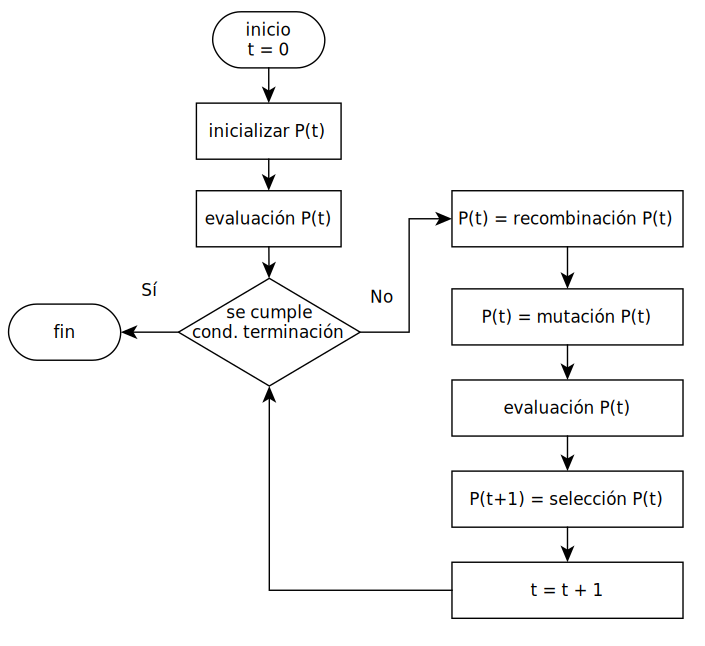
\includegraphics[scale=0.4]{EA_flowchart.pdf}

\end{frame}
%%%%%%%%%%%%%%%%%%%%%%%%%%%%%%%%%%%%%%%%%%%%%%%%%%%%%%%%%%%%%%%%%%%%%%%%%%%%%%%
\begin{frame}

\begin{block}{Ventajas}
\begin{itemize}
\item Problemas de optimización con espacio de búsqueda muy grande.
\item No requieren un análisis simbólico del problema.
\item Muy adecuados para Robótica.
\end{itemize}
\end{block}

\begin{block}{Inconvenientes}
\begin{itemize}
\item Pueden caer en óptimos locales.
\item No proporcionan una explicación de la solución.
\end{itemize}
\end{block}

\end{frame}
%%%%%%%%%%%%%%%%%%%%%%%%%%%%%%%%%%%%%%%%%%%%%%%%%%%%%%%%%%%%%%%%%%%%%%%%%%%%%%%

\begin{frame}
\frametitle{Introducción}
\begin{block}{Propósito}
\begin{itemize}
\item Lenguaje de programación orientado al cálculo numérico.
\item Objetivo: explotar al máximo la GPU y la CPU.
\end{itemize}
\end{block}
\end{frame}

\begin{frame}
\frametitle{QEA}


General	Purpose computing on Graphics Processing Units

Usar la GPU como herramienta de computación

\pause

SIMD = Single Instruction, Multiple Data

Ejecutar una sóla instrucción a varios elementos a la vez.

\pause

OpenCL = OpenComputing Language

Lenguaje para cálculo paralelo independiente del hw (2009).


\end{frame}



%%%%%%%%%%%%%%%%%%%%%%%%%%%%%%%%%%%%%%%%%%%%%%%%%%%%%%%%%%%%%%%%%%%%%%%%%%%%%%%%
\begin{frame}
\frametitle{Introducción a la computación cuántica (QC)}
Objetivo: Aprovechar las propiedades de la naturaleza en una escala muy pequeña, 
para realizar computaciones.

\pause

Motivación: La gran aceleración que se puede obtener y el bajo coste energético

\end{frame}
%%%%%%%%%%%%%%%%%%%%%%%%%%%%%%%%%%%%%%%%%%%%%%%%%%%%%%%%%%%%%%%%%%%%%%%%%%%%%%%%
\begin{frame}[t]
\frametitle{El bit frente al qubit}

%$$\frac{|0\rangle+i|1\rangle}{\sqrt{2}}$$
%$$\frac{|0\rangle+|1\rangle}{\sqrt{2}}$$
\begin{columns}
	\begin{column}{0.25\textwidth}
		\center
		Clásico
	\end{column}
	\begin{column}{0.25\textwidth}
		\center
		Clásico
	\end{column}
	\begin{column}{0.25\textwidth}
		\center
		Probabilístico
	\end{column}
	\begin{column}{0.25\textwidth}
		\center
		Cuántico
	\end{column}
\end{columns}

\begin{columns}[c]
	\begin{column}{0.25\textwidth}
		Estados
	\end{column}
	\begin{column}{0.25\textwidth}
		\includesvg[width=\textwidth]{bit}
	\end{column}
	\begin{column}{0.25\textwidth}
		\includesvg[width=\textwidth]{pbit}
	\end{column}
	\begin{column}{0.25\textwidth}
		\includesvg[width=\textwidth]{qbit}
	\end{column}
\end{columns}

\begin{columns}[b]
	\begin{column}{0.25\textwidth}
		Descripción
	\end{column}
	\begin{column}{0.25\textwidth}
		$$ \begin{bmatrix}
			1 \\
			0 \\
			\end{bmatrix} $$
	\end{column}
	\begin{column}{0.25\textwidth}
		$$ \begin{bmatrix}
			p \\
			1-p \\
			\end{bmatrix}
			\, p \in \mathbb{R} $$
	\end{column}
	\begin{column}{0.25\textwidth}
		$$ \begin{bmatrix}
			\alpha \\
			\beta \\
			\end{bmatrix} 
			\, \alpha, \beta \in \mathbb{C} $$
	\end{column}
\end{columns}

\end{frame}
%%%%%%%%%%%%%%%%%%%%%%%%%%%%%%%%%%%%%%%%%%%%%%%%%%%%%%%%%%%%%%%%%%%%%%%%%%%%%%%%
\begin{frame}
\frametitle{}

\end{frame}
%%%%%%%%%%%%%%%%%%%%%%%%%%%%%%%%%%%%%%%%%%%%%%%%%%%%%%%%%%%%%%%%%%%%%%%%%%%%%%%%



\begin{frame}
\frametitle{Dónde está la mejora? Ejemplo de matrices.}

$A, B$ y $C$ son matrices de $NxN$. Disponemos de $P$ núcleos.

Calcular $C = A * B$. Complejidad $ O(n^3) $.


\begin{itemize}
\item Dividir la matriz $C$ en bloques de $P$ elementos.
\item Asignar cada elemento $(i,j)$ del bloque a un núcleo:
\item Repetir para todos los bloques.
\end{itemize}

\end{frame}



\begin{frame}[fragile]
Procesamiento paralelo, en cada núcleo

\begin{lstlisting}

    C[i][j] = 0;
    for(k = 0; k < K; k++)
        C[i][j] += A[i][k] * B[k][j];

\end{lstlisting}

Complejidad final de $ O(n^3 / P) $

\end{frame}



\begin{frame}
\frametitle{Demo}
Multiplicación de matrices.
\end{frame}



\begin{frame}

\frametitle{Ejemplo de filtro.}

Cada núcleo ejecuta un pequeño programa, como sumar los valores
de los píxeles vecinos.

El resultado se almacena en un lugar aparte, sin modificar la original.

Todos los núcleos se pueden ejecutar en paralelo.

La imagen resultante, regresa a la RAM.

\end{frame}



%\begin{frame}
%\center
%\includegraphics[width=\textheight]{convolucion.jpg}
%\end{frame}



\begin{frame}
\frametitle{Problema}

Sabemos resolver muchos problemas, empleando algoritmos secuenciales.
Convertir un algoritmo a uno paralelo, requiere replantearlo.

\end{frame}



\begin{frame}[fragile]
\frametitle{Solución?}

Realizar cambios mecánicamente en el código secuencial para vectorizar aquello
que sea posible. Rama de investigación, vectorización.

Ejemplo:

\begin{lstlisting}
    for(i = 0; i < N; i++)
    {
        A[i]++;
        A[N-1-i]++;
    }
\end{lstlisting}

El optimizador debe ser capaz de deducir:

\begin{lstlisting}
A = A + 2;
\end{lstlisting}

\end{frame}



\begin{frame}
\frametitle{Optimización de código secuencial}
Tratar de paralelizar todo el código posible.

Crear un grafo de operaciones y simplificarlo.
\end{frame}



\begin{frame}[fragile]
Código de ejemplo

\begin{lstlisting}
 A = B*C + D*E
 C = A+E + E*B
 B = B*E + C
\end{lstlisting}

Descomposición:

\begin{lstlisting}
1    F = B*C
2    G = D*E
3    A = F+G
4    H = A*E
5    C = H+B
6    I = B*E
7    B = I*C
\end{lstlisting}

\end{frame}



\begin{frame}[fragile]
Descomposición:
\begin{lstlisting}
1    F = B*C
2    G = D*E
3    A = F+G
4    H = A*E
5    C = H+B
6    I = B*E
7    B = I*C
\end{lstlisting}
Tabla de operaciones:
\begin{lstlisting}
  A B C D E F G H I
  -----------------
1   . .     1      
2       . .   2        
3 3         . .        
4 .       .     4     
5   . 5         .
6   .     .       6
7   7 .           .
\end{lstlisting}
\end{frame}



\begin{frame}[fragile]
Tabla de operaciones:
\begin{lstlisting}
  A B C D E F G H I
  -----------------
1   . .     1      
2       . .   2        
3 3         . .        
4 .       .     4     
5   . 5         .
6   .     .       6
7   7 .           .
\end{lstlisting}
Optimización de operaciones.
\begin{lstlisting}
  A B C D E F G H I
  -----------------
1   . . . . 1 2    
2 3         . .       
3 .       .     4    
4   . 5   .     . 6
5   7 .           .
\end{lstlisting}
\end{frame}



\begin{frame}[fragile]
Optimización de operaciones.
\begin{lstlisting}
  A B C D E F G H I
  -----------------
1   . . . . 1 2    
2 3         . .       
3 .       .     4    
4   . 5   .     . 6
5   7 .           .
\end{lstlisting}
Optimización del espacio.
\begin{lstlisting}

  A B C D E F G H I
  -----------------
1   . . . . 1 2    
2 3         . .    
3 .       . 4      
4   . 5   . . 6    
5   7 .       .    
\end{lstlisting}
\end{frame}



\begin{frame}

\end{frame}



\begin{frame}
\center ¿Preguntas?
\end{frame}

\end{document}
